\documentclass[10pt,a4paper]{article}
\usepackage{amsmath}
\usepackage[
    colorlinks,
    citecolor=blue!70!black,
    linkcolor=blue!70!black,
    urlcolor=blue!70!black
]{hyperref}
\usepackage{tikz}
\usetikzlibrary{patterns}
\usepackage{xcolor}

\begin{document}

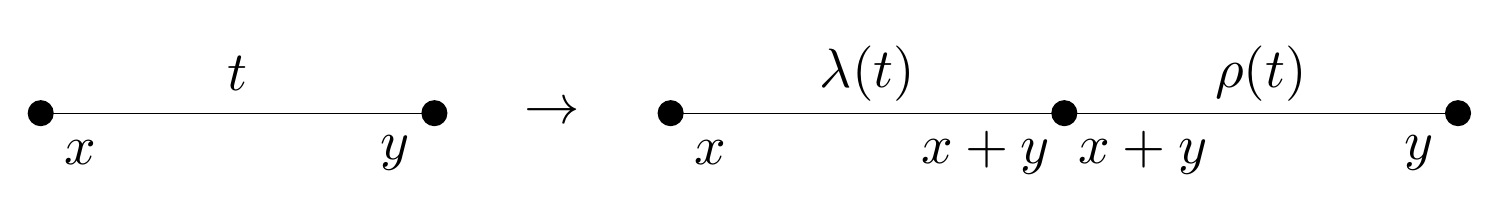
\begin{tikzpicture}
        \draw (-1,1) -- (4,1);
        \node[scale=1] at (-1,1) [circle,fill=black] {};
        \node[scale=1] at (4,1) [circle,fill=black] {};
        \node[scale=2] at (-.5,.5) {$x$};
        \node[scale=2] at (3.5,.5) {$y$};
        \node[scale=2] at (1.5,1.5) {$t$};

        \node[scale=2] at (5.5,1) {$\rightarrow$};

        \draw (7,1) -- (12,1);
        \node[scale=1] at (7,1) [circle,fill=black] {};
        \node[scale=1] at (12,1) [circle,fill=black] {};
        \node[scale=2] at (7.5,.5) {$x$};
        \node[scale=2] at (11,.5) {$x+y$};
        \node[scale=2] at (9.5,1.5) {$\lambda(t)$};

        \draw (12,1) -- (17,1);
        \node[scale=1] at (17,1) [circle,fill=black] {};
        \node[scale=2] at (13,.5) {$x+y$};
        \node[scale=2] at (16.5,.5) {$y$};
        \node[scale=2] at (14.5,1.5) {$\rho(t)$};
    \end{tikzpicture}

\end{document}